%        File: presenta.tex
%     Created: Mon Sept 16 11:00 AM 2019
% Last Change: Mon Sept 16 11:00 AM 2019
%
%      Author: Carlos Rodríguez

\documentclass[hyperref={pdfpagelabels=false},xcolor=pst,pdf,fragile]{beamer}


\providecommand\thispdfpagelabel[1]{}
\usepackage{lmodern}
\usepackage[utf8]{inputenc}
\usepackage{listings}
\usepackage{hyperref}
\usepackage{subfig}
%\usepackage[spanish]{babel}

%Copenhagen, Warsaw
\usetheme{Boadilla}
\usefonttheme{serif}

\def\Author{Carlos Rodríguez}
\def\Matricula{}
\def\Teacher{}
\def\Title{Hiperlordosis Lumbar}



\title{\Title}
\author{\Author\\ \Matricula}
\date{\today}

\begin{document}
\maketitle

\AtBeginSection[]
{
  \begin{frame}
    \frametitle{Outline}
    \tableofcontents[currentsection]
  \end{frame}
}

\AtBeginSubsection[]
{
  \begin{frame}
    \frametitle{Outline}
    \tableofcontents[currentsection,currentsubsection]
  \end{frame}
}

\section{¿Qué es la hiperlordosis lumbar?}

\begin{frame}
  \frametitle{
	  \href{http://www.espalda.org/divulgativa/dolor/causas/alteraciones/hiperlordosis.asp}
	  {Hiperlordosis Lumbar}
  }
  
  \pause
  \begin{itemize}
	\item Acentuación de la curvatura normal o fisiológica de la columna lumbar
  \end{itemize}
  
  \begin{center}
	  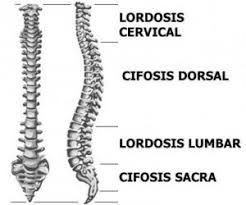
\includegraphics[scale=0.4]{img/columna_vertebral.jpeg}
  \end{center}

\end{frame}

\begin{frame}
  \frametitle{
	  {¿Cuál es la curvatura normal?}
  }

  \begin{center}
	  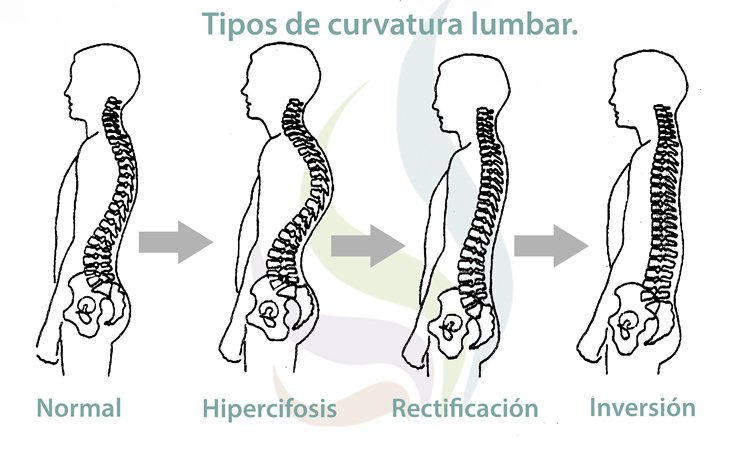
\includegraphics[scale=0.4]{img/tipos_de_curvatura.jpg}
  \end{center}

\end{frame}


\begin{frame}
  \frametitle{¿Cómo identificar la hiperlordosis?}

\begin{figure}
    \centering
    \pause
    \subfloat[]{{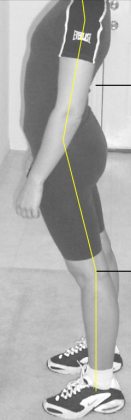
\includegraphics[width=2cm]{img/hiperlordosis_lumbar_ninio.png} }}
    \qquad
    \pause
    \subfloat[]{{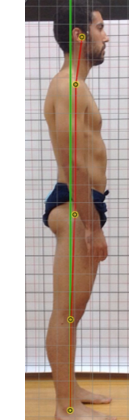
\includegraphics[width=2cm]{img/columna_normal.png} }}
    \qquad
    \pause
    \subfloat[]{{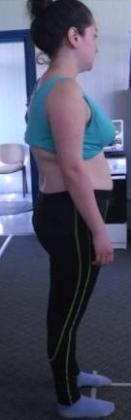
\includegraphics[width=2cm]{img/hiperlordosis_punto_inflexion.jpg} }}
    \caption{Ejemplos posturales}
    \label{fig:example}
\end{figure}

\end{frame}

\section{Signos y síntomas}
\begin{frame}
\frametitle{Sintomas}
  \begin{itemize}
	\item Dolor lumbar (interapofisarias) *hacer ejercicio de movimiento
	\item Dolor lumbar por contractura
	\item Artrosis
	\item Pinzamiento nervioso por deformidad articular
  \end{itemize}

  \pause

  Causados por:
  \begin{itemize}
	\item Disminución de espacio en articulaciones interapofisarias
	\item Hipertonía paravertebral o arco reflejo de irritación
	\item Desgaste debido a la constante fricción
	\item Disminución de espacio intervertebral, puede pellizcar médula ósea
  \end{itemize}

\end{frame}

\begin{frame}
  \frametitle{¿Qué músculos fijan la pelvis en anteversión y mantienen la hiperlordosis lumbar?}

  Imaginemos la pelvis como una polea:
    \begin{center}
	  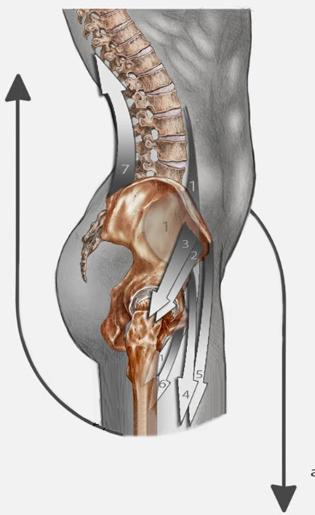
\includegraphics[scale=0.4]{img/pelvis_polea.jpg}
  \end{center}
\end{frame}

\begin{frame}
    \begin{center}
	  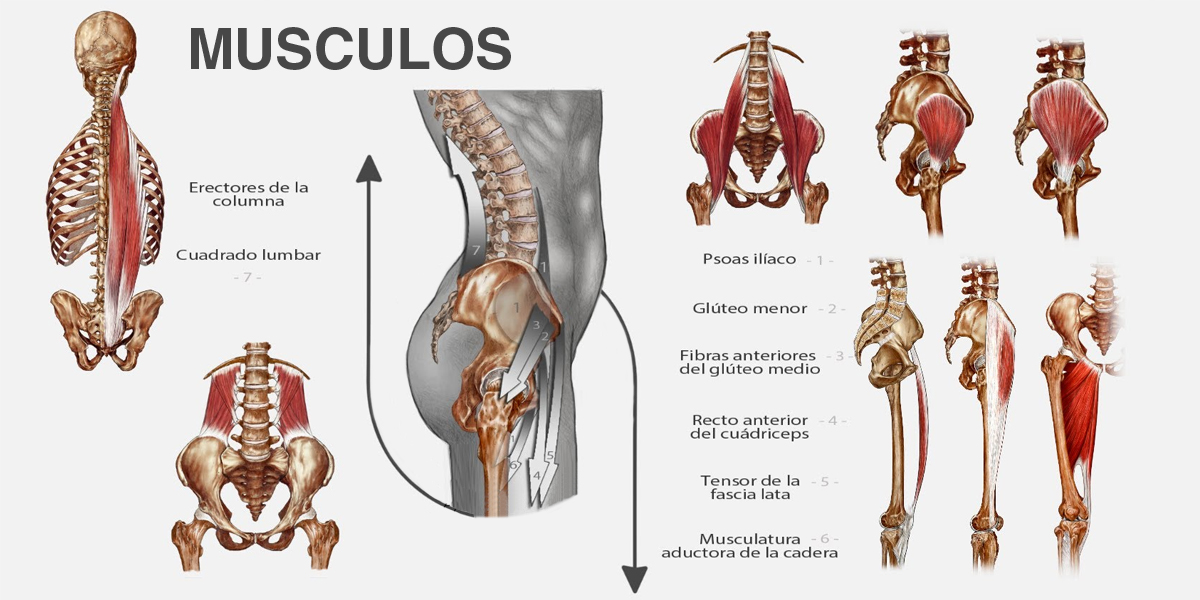
\includegraphics[scale=0.3]{img/musculos.jpg}
    \end{center}

\end{frame}

\section{Causas}
\begin{frame}
  \begin{itemize}
	\item Sobrepeso
	\pause
	\item Embarazo
	\pause
	\item Traslación anterior de la pelvis (carga en el antepie)
	\pause
	\item Tacones
	\pause
	\item Hipertonía de músculos erectores y/o cuadrado lumbar
	\pause
	\item Hipertonía/acortamiento de flexores de cadera
	\pause
	\item Rotación interna de cadera
	\pause
	\item Factores genéticos
  \end{itemize}

\end{frame}

\section{Correcciones}
\begin{frame}
  \begin{itemize}
	\item Apoyar el peso sobre toda la planta del pie
	\pause
	\item Evitar "acomodar" la pelvis
	\pause
	\item Estirar los músculos requeridos
	\pause
  \end{itemize}
\end{frame}

\begin{frame}[fragile]
  \frametitle{Estiramientos óptimos}
  \begin{itemize}
	\item Mejorar el equilibro pélvico (estirar flexores de cadera, musculatura paravertebral lumbar, estiramiento de cuadrado lumbar, estiramiento de aductores)
	\pause
	\item Tonificar abdominales
	\pause
  \end{itemize}

    \begin{block}{Open Definition} % alertblock, exampleblock
	  \begin{lstlisting}
Asegurar que las extensiones sean realizadas 
con un arco suave, y disminuir la carga sobre 
las articulaciones interapofisarias.

	  \end{lstlisting}
  \end{block}
  
\end{frame}

\begin{frame}
  \frametitle{Combinación de punto de inflexión + rectificación lumbar}
  \begin{itemize}
	\item Retrasar el centro de gravedad
	\pause
	\item Mejorar carga en superficie plantar
	\pause
	\item Descontracturar músculos erectores de la región del punto de inflexión
  \end{itemize}
\end{frame}


\end{document}


